\section{Ex. 3.3: Halloween storm evolution}

Analyze the ionospheric delays for 6 consecutive days including the Halloween storm:

\begin{enumerate}
\item This is a simple exercise aimed to illustrate the ionospheric delay variation during the Halloween storm. A period of 6 consecutive days (from October 28 to November 2, 2003) are analyzed using measurements collected in the “garl” station in North America.
\item The STEC variations are depicted from the geometry-free combination of codes P2-P1.
\end{enumerate}

Note that:
\begin{equation}\label{Geometry free combination}
    P_{2}-P_{1} = I +K_{21}
\end{equation}


\textcolor{red}{BUG HERE}
\begin{figure}[H]
        \centering
        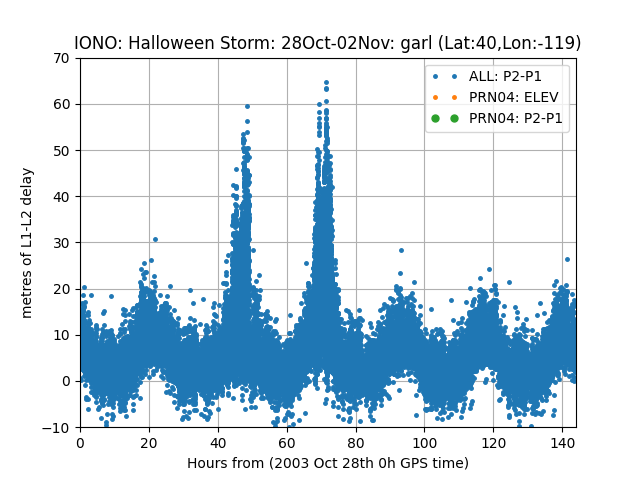
\includegraphics[scale=0.52]{sources/Figures/FIG_2/TUT2_Ex3.3c.png}
        \caption{}
        \label{fig:}
\end{figure}

\textcolor{red}{BUG HERE}
\begin{figure}[H]
        \centering
        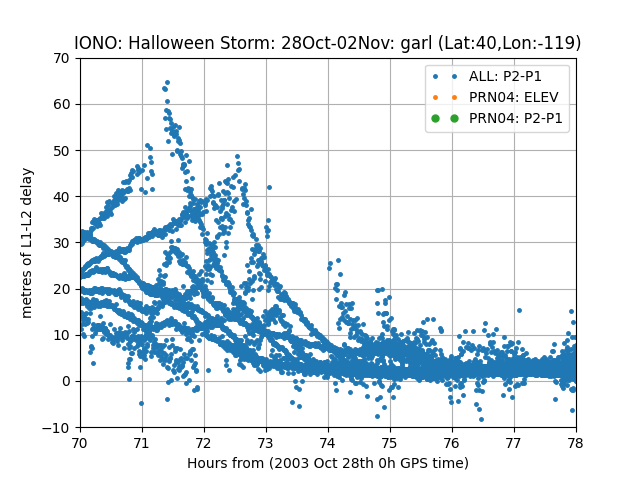
\includegraphics[scale=0.52]{sources/Figures/FIG_2/TUT2_Ex3.3d.png}
        \caption{}
        \label{fig:}
\end{figure}

\begin{enumerate}
\item What is the maximum STEC seen before and after the storm? And during the storm?
\item The STEC of satellite PRN04 shows a flat pattern after time 74 hours which does not change with the elevation. Try to explain this phenomenon.
\end{enumerate}